\documentclass[addpoints]{exam}
\usepackage{url}
\usepackage{amsmath,amsthm,enumitem}
\usepackage{graphicx}
\usepackage{qtree}
\usepackage[nodayofweek,level]{datetime}
\usepackage{color}
\usepackage{csquotes}
\usepackage{pgf, tikz}
\usetikzlibrary{arrows, automata}
\usepackage{algorithm,algpseudocode}

\definecolor{qcolor}{rgb}{0, 0, 0.3}
\definecolor{acolor}{rgb}{0, 0, 0}
%\input myfonts

\lhead{Gopal Menon (u0772360)}
\chead{\bf{HW2}}
\rhead{CS 6150 \today}
\headrule

\begin{document}

\section*{Collaborators}

Ben Nelson and I collaborated for this assignment on all questions except $3$.

\begin{questions}
\titledquestion{Coin change revisited}
In class, we saw the ``coin change'' problem, where we have $k$ types of coins, of denominations $d_1, d_2, \dots, d_k$ resp., and the goal is to make change for $N$ cents using the minimum {\em number} of coins (here $N, d_1, \dots, d_k$ are given positive integers). 

We saw that a greedy strategy does not work, and we needed to use dynamic programming.
\begin{parts}
\part[3] We discussed a dynamic programming algorithm that uses space $O(N)$ and computes the minimum number of coins needed. Give an algorithm that improves the space needed to $O(\max_i (d_i))$. 

The issue with a greedy approach to this problem is that sometimes the best solution is using coins where the highest denomination coin is not used up first. For example if the set of coins is $\{1,3,4,5\}$ and we need to find the minimum number of coins that add up to $7$, a greedy approach would lead us to use $5$ first followed by two coins of denomination $1$. This would mean using up $3$ coins, but the optimum solution is $2$ coins where we use $3$ and $4$. To get around this problem we could use multiples of the largest denomination coin to get the required total $N$ to a number not less than twice the value of the largest denomination coin. Then we can use the $O(N)$ space algorithm to compute the minimum number of coins required for the remaining amount that was the number not less than twice the value of the largest denomination coin. The algorithm is detailed below with \Comment{} identifying comments.

\let\oldReturn\Return
\renewcommand{\Return}{\State\oldReturn}

\begin{minipage}{\linewidth}
  \begin{algorithm}[H]
    \caption{Minimum Number of Coins}\label{AlgPeck}
    \begin{algorithmic}[1]
      \Procedure{MinimumNumberofCoins}{$Total\_Cents$, $Denominations\_List$}
      	\State $largest\_coin\_count = \frac{Total\_Cents-2 \times max(d_i)}{max(d_i)}  $ \Comment{ integer division is used}
	\State $Minimum\_Number\_of\_Coins =$ 
	\State \text{       }$Big\_Oh\_N\_Space\_Algorithm(N-largest\_coin\_count \times max(d_i), Denominations\_List) $
	\Return $Minimum\_Number\_of\_Coins + largest\_coin\_count $ 
      \EndProcedure
    \end{algorithmic}
  \end{algorithm}
\end{minipage}\\\\

In the case of the coin denominations $\{1,3,4,5\}$, for a total of 28 cents, we would first find how many of the largest denomination coins can be used up to bring the total to be  not less than twice the value of the largest denomination coin. By using three $5$ cent coins, we can bring the total down to $28-3\times5=28-15=13$. Then we use the $O(N)$ space complexity algorithm to find the minimum number of coins for the remaining amount. Here $O(N)$ will be $O(2\times max(d_i))=O(max(d_i))$. The algorithm space complexity is thus $O(max(d_i))$.


\part[5] Design an algorithm that outputs the number of different ways in which change can be obtained for $N$ cents using the given coins. (Two ways are considered different if they differ in the number of coins used of at least one type.) Your algorithm needs to have time and space complexity polynomial in $N, k$.

\begin{minipage}{\linewidth}
  \begin{algorithm}[H]
    \caption{Coin Change Ways}\label{AlgPeck}
    \begin{algorithmic}[1]
    	\State
      	\State $change\_ways = 0$ \Comment{coin change ways count}
	\State $change\_ways\_for\_amount = new array[N]$ \Comment{coin change ways per amount}
	\State initialize $change\_ways\_for\_amount$ array with null values
	\State CoinChangeWays($N$, $\{d_1, d_2, \dots, d_k\}$)
	\State Print $change\_ways$
	\State
      \Procedure{CoinChangeWays}{$Total\_Cents$, $Denominations\_List$}
      	\State
      	\If {$Total\_Cents==0$}
      		\State return $1$
	\EndIf
    	\State
	\For {coin $d_i$ in $\{d_1, d_2, \dots, d_k\}$}
	    	\State
		\If {$Total\_Cents < d_i$}
			\State continue \Comment{Skip this coin as it cannot be used}
		\EndIf
	    	\State
		\State max\_coin\_count = $\frac{Total\_Cents}{d_i}$ \Comment{Integer division}
	    	\State
		\For {$coins\_used$ in range 1 to max\_coin\_count}
		    	\State
			\State $new\_total\_cents = Total\_Cents - coins\_used \times d_i$
			\If {$change\_ways\_for\_amount[new\_total\_cents] $ \text{ is null}}
				\State $change\_ways\_for\_amount[new\_total\_cents] $= 
				\State \text{         }CoinChangeWays($new\_total\_cents$, $Denominations\_List$)
			\EndIf
		    	\State
			\State $change\_ways = change\_ways + change\_ways\_for\_amount[new\_total\_cents]$
		    	\State
		\EndFor
	    	\State
	\EndFor
      \EndProcedure
    \end{algorithmic}
  \end{algorithm}
\end{minipage}\\\\

The algorithm for Coin Change Ways has $change\_ways$ and $change\_ways\_for\_amount$ as global variables and uses dynamic programming to recurse through all possible usages of the coins collection to get the total change required. It uses an array to store intermediate values and the total space complexity is the size of the array, which is $O(N)$. Although this is a recursive algorithm, due to memoization, each amount between $1$ and $N$ is computed only once. Since we loop through each of the $k$ coins once and for each coin we do a maximum of $N$ computations, the time complexity of the algorithm is $O(kN)$.


\end{parts}


\titledquestion{Counting paths}
Directed acyclic graphs, or DAGs, are graphs that show up in many applications. A directed graph $G$ is called a DAG if it has no directed cycles. Given a DAG $G$ on $n$ vertices, and an integer $k < n$, 

\begin{parts}
\part[5] Design an algorithm that counts the number of paths of length $k$ in $G$.  {\bf Prove that your algorithm runs in time polynomial in $n$ and $k$.}
\part[2] Explain (in a couple of sentences) what goes wrong when $G$ has directed cycles.
\end{parts}


\begin{parts}

\part I will start with an example of a DAG that has been topologically sorted in the order $a$, $b$, $c$ and $d$ as shown below. A topological sort can be done in $O(|V|+|E|)$ \cite{CLRS} where $V$ is the set of vertices and $E$ is the set of edges in the graph. After a topological sort is done, the nodes will be picked up in the order from left to right, and for each node the number of paths leading out and their corresponding path lengths will be stored. This will be done recursively along with memoization. Since a topological sort is done first, we know that there will not be any edges going back and we only need to look at the edges going forward.

\begin{center}
  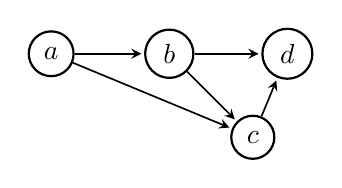
\begin{tikzpicture}[
            > = stealth, % arrow head style
            shorten > = 1pt, % don't touch arrow head to node
            auto,
            node distance = 1.5cm, % distance between nodes
            semithick % line style
        ]

        \tikzstyle{every state}=[
            draw = black,
            thick,
            fill = white,
            minimum size = 4mm
        ]

        \node[state] (a) {$a$};
        \node[state] (b) [right of=a] {$b$};
        \node[state] (c) [below right of=b] {$c$};
        \node[state] (d) [right of=b] {$d$};

        \path[->] (a) edge node {} (b);
        \path[->] (a) edge node {} (c);
        \path[->] (b) edge node {} (c);
        \path[->] (b) edge node {} (d);
        \path[->] (c) edge node {} (d);

  \end{tikzpicture}
\end{center}

Due to the nature of the recursive algorithm, the last node will be processed first. Every node will memoize a data structure corresponding the number of forward paths. In the case of the above DAG that has been topologically sorted, node $d$ will be picked up first. Since there are no outgoing edges, it will memoize a null for the forward paths information. The recursive call will then return to the recursion level corresponding to node $c$. For each forward node from $c$, it will create an entry for a path of length one in the memoized data structure and will make copy of the path lengths memoized at node $d$ and add $1$ to each path length and store that too in the memoized data structure. \\

Since no forward path information was returned from node $d$, the $c$ will memoize $\{\{length=1, paths=1\}\}$ to say that there is $1$ forward path of length $1$ from node $c$. The recursion level for node $b$ will create an entry $\{length=1, paths=2\}$ in the memoized data structure corresponding to the node $b$ corresponding to the $2$ forward paths of length $1$ from node $b$ to the two nodes $c$ and $d$. Then the two path lengths memoized in the forward nodes $c$ and $d$ will be merged and $1$ will be added to each path length. This will result in $\{length=2, paths=1\}$, which will also be memoized to give the updated memoized data structure corresponding to node $b$ $\{\{length=1, paths=2\}, \{length=2, paths=1\}\}$ to say that there are $2$ paths of length $1$ from $b$ corresponding to the paths to $c$ and $d$ and $1$ path of length $2$ corresponding to the path from $b$ to $c$ to $d$. Finally the recursion level for node $a$ will memoize $\{length=1, paths=2\}$ corresponding to length $1$ paths to  $b$ and $c$. Then it will retrieve the memoized entry for $b$ $\{\{length=1, paths=2\}, \{length=2, paths=1\}\}$ and add $1$ to each path length to give $\{\{length=2, paths=2\}, \{length=3, paths=1\}\}$. This will then be added to the memoized entry for $a$ to give $\{\{length=1, paths=2\}, \{length=2, paths=2\}, \{length=3, paths=1\}\}$.\\

Once the memoized entry for each node is available, we can look at each node, count the number of paths of length $k$ starting at each node, and add up all the intermediate sums to get the number of paths of length $k$ in the entire graph. Here is the algorithm:

\begin{minipage}{\linewidth}
  \begin{algorithm}[H]
    \caption{Count Paths of Length}\label{}
    \begin{algorithmic}[1]
      \Procedure{CountPathsOfLength}{Graph $G \{V, E\}$, Length $k$}
    	\State Do topological sort for graph $G$ to get $sorted\_indexes$
	\State $path\_lengths$ = [$|V|$] \Comment{array with $|V|$ elements}
	\State Initialize $path\_lengths$ with nulls
      	\State GetPathsLengths($G$, $sorted\_indexes$, 1, $path\_lengths$, k)
	\State return PathLengthsEqualTo(k)
      \EndProcedure
      \Procedure{GetPathsLengths}{Graph $G$, $sorted\_indexes$, $index\_number$, $path\_lengths$, k}
	\If {$index\_number == |V|$} \Comment{last node}
		\State $path\_lengths[index\_number] = null$
		\State return
	\EndIf
    	\State $next\_node\_path\_lengths$ 
      	\State \text{         } = GetPathsLengths($G$, $sorted\_indexes$, $index\_number+1$, $path\_lengths$)
	\State \text{Merge path lengths stored in next nodes with } $next\_node\_path\_lengths$  
      	\State $next\_node\_paths =\{length=1, paths = \text{number of next nodes}\}$
      	\State $\text{Increase paths lengths in } next\_node\_path\_lengths \text{ by 1} \text{ if not null and limited to k}$ 
      	\State $\text{Store above two paths lengths in }path\_lengths[index\_number] $ \Comment{memoize path lengths}
	\State return $path\_lengths[index\_number] $
      \EndProcedure    
      \Procedure{PathLengthsEqualTo}{Graph $G$, $path\_lengths$, $k$}
      	\State $number\_of\_paths = 0$
	\For {$path\_length$ in $path\_lengths$}
		\State $number\_of\_paths = number\_of\_paths + \text{ k length paths in path\_length} $
	\EndFor
      	\State return $number\_of\_paths$
      \EndProcedure    
     \end{algorithmic}
  \end{algorithm}
\end{minipage}\\\\

\textbf{Run time analysis of algorithm: } As described earlier, the topological sort can be done in $O(|V| + |E|)$ time. Creating the $path\_lengths$ array and initializing it can be done in $O(|V|)$ time. The $GetPathsLengths$ procedure will be called once for every node. If every node has $O(\frac{|E|}{|V|})$ forward edges, then the amount of work involved in running the $GetPathsLengths$ procedure on all nodes will be $O(\frac{|E|}{|V|}\{1+2+3+\ldots+k+k+k\})$. The reason for the $k$'s is that once we reach path length of k, we do not need to count further. So the amount of work in the procedure calls is $O(\frac{|E|}{|V|}k^2) = O(\frac{|V|^2}{|V|}k^2)= O(|V|k^2)$. Here we have used $|E| = O(|V|^2)$. The procedure $PathLengthsEqualTo$ will do $O(|V|)$ work since it looks at the path lengths at every node. So the total work done by the algorithm is $O(|V| + |E| + |V|k^2) = O(|V| + |V|^2 + |V|k^2) = O(|V|(|V|+k^2) = O(n(n+k^2))$ since $|V| = n$. This shows that the time complexity of the algorithm is a polynomial in $n$ and $k$

\part If the $G$ has directed cycles, then a topological sort cannot be done and the algorithm described above will not work. Also if the graph has cycles, then any path length can be found if you keep going in a cycle.

\end{parts}

\titledquestion{The Ill-prepared Burglar}
Suppose a burglar breaks into a house, and realizes the house has far too many items to fit into his sack. He thus wishes to pick the items of most value that he can end up taking. To formalize, the house has $n$ objects, and the $i$th object has value $v_i$ and size $s_i$.  The burglar has a sack that has a total size $S$.
\begin{parts}
\part[2] Not being trained in algorithms, he starts stuffing items into his sack, in decreasing order of value. He stops when none of the items left can fit into his back. Give an example in which this strategy is not optimal.
\part[3] After obvious disappointment at his performance, the burglar decides to empty his sack and pick items in decreasing order of the {\em ratio} value/size. Give an example in which even this strategy is not optimal.
\end{parts}

\begin{parts}

\part Consider the case shown in the table below where the first two highest value items will fill the sack and give the burglar a total value of $50+30=80$. However if the burglar had instead stolen the next $6$ items, he would have got a value of $25\times 6=150$. This is an example of when stuffing items into his sack in decreasing order of value is not optimal.

\begin{center}
  \begin{tabular}{ |c |c|}
    \hline
    Item Value & Item  Size \\ \hline
   50& $S/2$  \\ \hline
    30 & $S/2 $ \\ \hline
    25 & $S/10 $ \\ \hline
    25 & $S/10 $ \\ \hline
    25 & $S/10 $ \\ \hline
    25 & $S/10 $ \\ \hline
    25 & $S/10 $ \\ \hline
    25 & $S/10 $ \\ 
    \hline
  \end{tabular}
\end{center}

\part Consider the case shown below for which the burglar picks items in decreasing order of the {\em ratio} value/size. He will pick up the first item in the table and will not be able to fit any other item. He will get a total value of $90$. On the other hand, if he had picked the last $3$ items in the table, he would have got a total value of $100$. This is an example of when stuffing items into his sack in decreasing order of the {\em ratio} value/size is not optimal.

\begin{center}
  \begin{tabular}{ |c|c|c|}
    \hline
    Item Value & Item  Size & Value/Size\\ \hline
   90& $3S/4$ & 120/S\\ \hline
    70 & $2S/3 $ & 105/S\\ \hline
    100/3 & $S/3 $ & 100/S\\ \hline
    100/3 & $S/3 $ & 100/S\\ \hline
    100/3 & $S/3 $ & 100/S\\ 
    \hline
  \end{tabular}
\end{center}


\end{parts}
\titledquestion{Road tripping}
Let us roll back to the days when a road trip meant writing all your favorite music onto CDs and carrying them along.

Suppose we have $n$ songs, of durations $d_1, d_2, \dots, d_n$, where each $d_i$ is less than one hour. Suppose that every CD can hold one hour of music. The goal is to write all the songs to a set of CDs, so as to minimize the number of CDs required.

Consider the natural greedy algorithm for the problem: at every step, we have a list of CDs containing the music written so far (initially empty). Now consider the songs in the given order, and for song $i$, write it to the first CD so far that has sufficient space for the song. If there is no such CD, then we buy a new CD, and write song $i$ to it (and add it to the CD list).

\begin{parts}
\part[3] Give an example in which the greedy algorithm is not optimal.

Consider the case where the order of songs with the lengths in minutes is $\{40,50,10,20\}$. The greedy algorithm will put the songs into the CDs in the following manner, where the numbers represent the steps where the next song is picked up:

\begin{enumerate}

\item CD1: $\{40\}$
\item CD1: $\{40\}$, CD2: $\{50\}$. A new CD is used since each CD has a capacity of only $60$ minutes and the $2$ songs will not fit on $1$ CD.
\item CD1: $\{40,10\}$, CD2: $\{50\}$. The song of length $10$ minutes will be written on the first CD with available space.
\item CD1: $\{40,10\}$, CD2: $\{50\}, CD3: \{20\}$. The song of length $20$ minutes will be written onto a new CD since it will not fit onto either of the first two CS.

\end{enumerate} 

The greedy algorithm will end up using $3$ CDs for a total song length of $120$ minutes or $2$ hours. An optimal algorithm would have stored the songs in the following manner: CD1: $\{40,20\}$, CD2: $\{50,10\}$ with just $2$ CDs used to fit the songs.

\part[7] Prove that the greedy algorithm is always within a factor $2$ of the ``best possible'' number of CDs. [{\em Hint: } You may want to compare the number of CDs used by the algorithm with the ``total duration'' of the songs.  Also, play around with small examples to see how the algorithm is doing.]
\end{parts}

If  the songs are not ordered in a fashion that will cause the greedy algorithm to use up the space in the CDs in an optimal fashion, there will always be wasted space on the CDs. 

\begin{equation*}
\begin{aligned}
\text{Space used by greedy algorithm} = G &= \sum_i d_i + \text{wasted space}\\
\end{aligned}
\end{equation*}

In the worst case performance of the greedy algorithm, each song will use up one CD with unused space of slightly less than $30$ minutes left on each CD. In the usual case however, the greedy algorithm may leave unused space that will be of less duration than that of the smallest length song. Based on this, we can say that:

\begin{equation*}
\begin{aligned}
G &= \sum_i d_i + \text{wasted space}\\
&\leq \sum_i d_i + \sum_i d_i - \epsilon \text{, where $\epsilon$ is a small quantity}\\
\Rightarrow G &\leq \sum_i d_i + \sum_i d_i \\
G &\leq 2 \sum_i d_i 
\end{aligned}
\end{equation*}

The optimum number of CDs will be lower bound by the total songs duration divided by the capacity of each CD

\begin{equation*}
\begin{aligned}
OPT &\geq  \frac{\sum_i d_i }{1}\\
OPT &\geq \sum_i d_i \\
\Rightarrow G &\leq 2 \times OPT \qed
\end{aligned}
\end{equation*}

\titledquestion{Maximizing Happiness}
Recall the matching problem we saw in class: there are $n$ gifts, and $n$ children, and each child has a non-negative valuation for each gift. Formally, the value of gift $j$ to child $i$ is given by $H_{i,j}$.  We assume that all $H_{i,j} \ge 0$. Santa's goal is to give one gift to each child, so as to maximize the {\em total value} (of course, a gift cannot be given to more than one child).

\begin{parts}
\part[3] We saw in class that starting with any assignment and performing swaps that improve the total value, we get to a solution whose cost is $\ge (1/2) \cdot OPT$, where $OPT$ is the cost of the optimum assignment of gifts. Prove that the factor $1/2$ cannot be improved in general.  I.e., give an instance and a starting solution, for which the locally optimum solution is a factor 2 worse than $OPT$. 

\part[7] Suppose we now perform a more elaborate local search, this time picking every {\em triple} of edges in the current solution, and seeing if there is a reassignment of gifts between the end points of these edges that can improve the total value. Prove that a locally optimal solution produced this way has a value that is at least $(2/3)$ the optimum value. [This kind of a trade-off is typical in local search -- each iteration is now more expensive $O(n^3)$ instead of $O(n^2)$, but the approximation ratio is better.]
\end{parts}
{\bf Note.}  We will see in the coming lectures that this problem can indeed be solved optimally in polynomial time, using a rather different algorithm. 

\begin{parts}

\part The following table shows the happiness values for when gifts $\{i,j,k,l\}$ are assigned to children $\{p,q,r,s\}$.

\begin{center}
  \begin{tabular}{ |c|c|c|c|c|}
    \hline
     &  $p$ & $q$ & $r$ & $s$\\ \hline
$i$  & $100$ & $50$  & $5$ & $0$\\ \hline
$j$  & $5$ & $100$  & $0$ & $50$\\ \hline
$k$    & $50$ & $0$  & $100$ & $5$\\ \hline
$l$    & $0$ & $5$ & $50$ & $100$\\ 
    \hline
  \end{tabular}
\end{center}

Suppose that a greedy algorithm assigns gifts $\{i,j,k,l\}$ to children $\{p,q,r,s\}$ in the following manner. The format is $H_{child_i, gift_j}$ for happiness score when $child_i$ is given $gift_j$.

\begin{equation*}
\begin{aligned}
H_{Total} &= H_{i,r}+H_{j,p}+H_{k,s}+H_{l,q}\\
&=5+5+5+5\\
&=20
\end{aligned}
\end{equation*}

We can start doing a local search by swapping gifts for two children at a time if this results in a higher happiness score. If the gifts assigned to children $i$ and $l$ are swapped, the total happiness becomes $110$. So this swap can be made. 

\begin{equation*}
\begin{aligned}
H_{Total} &= H_{l,r}+H_{j,p}+H_{k,s}+H_{i,q}\\
&=50+5+5+50\\
&=110
\end{aligned}
\end{equation*}

Now if the gifts assigned to children $j$ and $k$ are swapped, the total happiness becomes $200$. So this swap can be made. 

\begin{equation*}
\begin{aligned}
H_{Total} &= H_{l,r}+H_{k,p}+H_{j,s}+H_{i,q}\\
&=50+50+50+50\\
&=200
\end{aligned}
\end{equation*}


At this state, the total happiness will not increase (may remain the same) after any other swaps. So the local search is limited to a total happiness value of $200$. The optimum assignment of gifts for maximum total happiness is:

\begin{equation*}
\begin{aligned}
H_{Optimum} &= H_{i,p}+H_{j,q}+H_{k,r}+H_{l,s}\\
&=100+100+100+100\\
&=400
\end{aligned}
\end{equation*}

So the local optimum solution shown above is a factor $2$ worse that the optimum solution OPT.

\part Consider a triple from a set of assignments of gifts to children. In this case, the children $\{i,j,k\}$ are assigned gifts $\{p_i,o_i, q_i\}$ respectively, whereas the optimum gift assignment to these children would have been $\{q_i,p_i,o_i\}$. This means that

\begin{equation*}
\begin{aligned}
H_{i, p_i}+H_{j,o_i}+H_{k,q_i} &\geq H_{i, q_i}+H_{j,p_i}+H_{k,o_i}\\
\Rightarrow H_{i, p_i}+H_{j,o_i}+H_{k,q_i} &\geq H_{i, q_i}+H_{j,p_i}\\
\Rightarrow \sum_i H_{i, p_i}+\sum_i H_{j,o_i}+\sum_i H_{k,q_i} &\geq \sum_i H_{i, q_i}+\sum_i H_{j,p_i} \text{, summing over all $i$}\\
\Rightarrow 3 \times G &\geq 2 \times OPT\\
\Rightarrow G &\geq \frac{2}{3} \times OPT \qed
\end{aligned}
\end{equation*}
since each left term three lines above is the greedy solution and each right term is the optimum solution

\end{parts}

\titledquestion{Reverse greedy}[5]

Consider the following {\em reverse greedy} algorithm for the spanning tree problem: we start with the input graph $G$, and in each step, remove the edge of the largest weight that does not disconnect $G$.  The algorithm terminates when there is no such edge (i.e., what remains is a tree). Prove that this algorithm also finds the minimum weight spanning tree.

[{\em Hint: } Argue one step at a time (i.e., that the cost of the MST is preserved in each step). Prove this by contradiction. You may also want to use the observation that removing any edge of a tree divides the set of vertices it into two \underline{connected} pieces. ]

\textbf{Argument 1:} Consider the possibility that the cost of the MST is not preserved in a step. When an edge is removed as per the above algorithm, since the graph is still connected, there has to be at least one other path between the two nodes that the edge was removed from. Such a path will have at least two edges (if we assume that there is at most one edge between any two nodes). Let these edges be denoted by $\{e_1,e_2,\ldots,e_n\}$ and let the removed edge be denoted by $z$. Any MST will need to have a path between the two nodes that the edge was removed from. This path can be either through edge $z$ or through edges $\{e_1,e_2,\ldots,e_n\}$. There can be many such paths not through $z$. The following argument will cover all such paths.

Consider the case where all the edges in $\{e_1,e_2,\ldots,e_n\}$ were not larger than $z$. Then $|\{e_1,e_2,\ldots,e_n\} \backslash e_x \bigcup z| \geq \sum_i| e_i|$. ie. The sum of the length of all but any one edges in $\{e_1,e_2,\ldots,e_n\}$ and $z$ will be more than the sum of all the edges in $\{e_1,e_2,\ldots,e_n\}$. So in this case, by removing $z$, the MST cost does not increase.

Consider the other case where $\{e_1,e_2,\ldots,e_n\}$ had an edge or edges larger that $z$. This can only be the case where removing them would have disconnected the graph. In this case, removing $z$ would be the only option and so the MST cost does not increase by removing $z$ as this was the only option.

This means that the MST cost is preserved in each step. Clearly the base case, where no edges have been removed, will have an MST comprised of a subset of the edges. So this means by induction that the algorithm produces a MST.

\textbf{Argument 2 (alternate argument):} Consider the step of removing the largest length edge as described in the algorithm. Reorder the graph so that the nodes and edges connected to one end of the edge being removed are on one side and the nodes and edges connected to the other end of the edge being removed are on the other side. So we will have two sub-graphs connected by the edge being removed. If removing the edge had disconnected the graph, this edge would be the only connection between otherwise two separate graphs. Since removing the edge does not disconnect the graph, there will be at least one more edge between the two sub-graphs. So it is clear that at each step, removing the largest edge that does not disconnect the graph, preserves the cost of the MST.The reason is that there is at least one more path between the two sub-graphs and by removing the larger one, we would have removed an edge that could not have been in an MST as another smaller edge would have connected the two sub graphs. 

Clearly the base case, where no edges have been removed, will have an MST comprised of a subset of the edges. So this means by induction that the algorithm produces a MST.

\titledquestion{Uniqueness of spanning trees}[5]
Let $G$ be a connected, weighted, undirected graph in which all the edges have distinct weights. Prove that $G$ has a unique MST (minimum spanning tree), i.e., there is precisely one tree that achieves the minimum weight.  [{\em Note:}  this is a well-known fact (and you will likely find solutions online). But it is one you should know, and is not too hard to prove.]

[{\em Hint: } Suppose there are two minimum spanning trees $T$ and $T'$, and suppose their edges are $e_1, e_2, \dots, e_{n-1}$ and $f_1, f_2, \dots, f_{n-1}$ respectively, in increasing order of weights.  Consider the first $i$ for which $e_i \neq f_i$, and try to arrive at a contradiction. ]

Suppose there are two minimum spanning trees $T$ and $T'$, and suppose their edges are $e_1, e_2, \dots, e_{n-1}$ and $f_1, f_2, \dots, f_{n-1}$ respectively, in increasing order of weights. Consider the first $i$ for which $e_i \neq f_i$. This means that either $e_i < f_i$ or $e_i > f_i$ since all edge weights are unique. Since the edges are sorted in increasing order of weights, the tree where the edge is larger, will clearly have a higher weight than the other tree, since all edge weights for the tree after $i$ will be larger than the weight at position $i$. So the tree with the higher sum of weights is clearly not a \textit{Minimum} Spanning Tree even though it may be a Spanning Tree since the other tree has a lower sum of weights. If there is no $i$ where $e_i \neq f_i$, it means that both the trees are identical. So that means that the MST is unique.

\end{questions}


\begin{thebibliography}{9}

\bibitem{CLRS} \enquote{22.4 Topological sort.} \textit{Introduction to Algorithms}, by Thomas H. Cormen et al., Mit Press, 2009, pp. 613-613.

\end{thebibliography}

\end{document}
